\chapter{Configuration of Linux TC}
\label{ch:tc}

This chapter covers the specifics of how the routing, queuing, and
shaping of network traffic is configured and how this traffic passes
through the queues and shapers in the Linux Kernel before being
transmitted through the network interface.

We configure the system's static routes using the Linux's built-in
IPRoute\cite{linux_iproute} tool, which allows for the configuration
of the kernel's routing tables, network address translation (NAT), and
characteristics of the network interface such as the maximum transmit
unit (MTU).  For each node, a route is added to the routing table
specifying the next hop address as its gateway for each other node to
which it is not directly connected.  In this way, the packets in the
network will be routed using loose source-based routing where the
sender node does not know the full route that the packet will take,
but just forwards it to the next known location.

The system's priority-based network traffic queuing, network delay,
and network bandwidth capacity was configured using Linux's built-in
Traffic Control (TC)\cite{linux_tc} tool (which is part of IPRoute),
that allows for the configuration of hierarchical class-based traffic
scheduling, and traffic shaping.  We configured the output interfaces
on each node as a combination of two queuing disciplines (qdiscs): 1)
a network emulator (netem) which enforces the link delay, and 2) a
token-bucket filter (TBF) which enforces the rate control to enforce
the link's bandwidth profile.  On the routing node, we added an
additional priority qdisc (prio), with multiple priority queues.  We
configured TC to filter packets into these queues by matching packet
source IP address and destination IP address.  This filtering ensured
that the high priority flow's packets would be filtered into the
high-priority queue of the prio qdisc, while the lower priority flow's
packets would be filtered into the lower priority queue of the prio
qdisc.  All traffic out of the priority qdisc was fed into the TBF to
ensure that all traffic, regardless of priority, shared and was shaped
by the node's link capacity profile.  The configuration and function
of TC is shown in Figure~\ref{fig:tc_diagram}.

\begin{figure}[ht!]
  \centering
  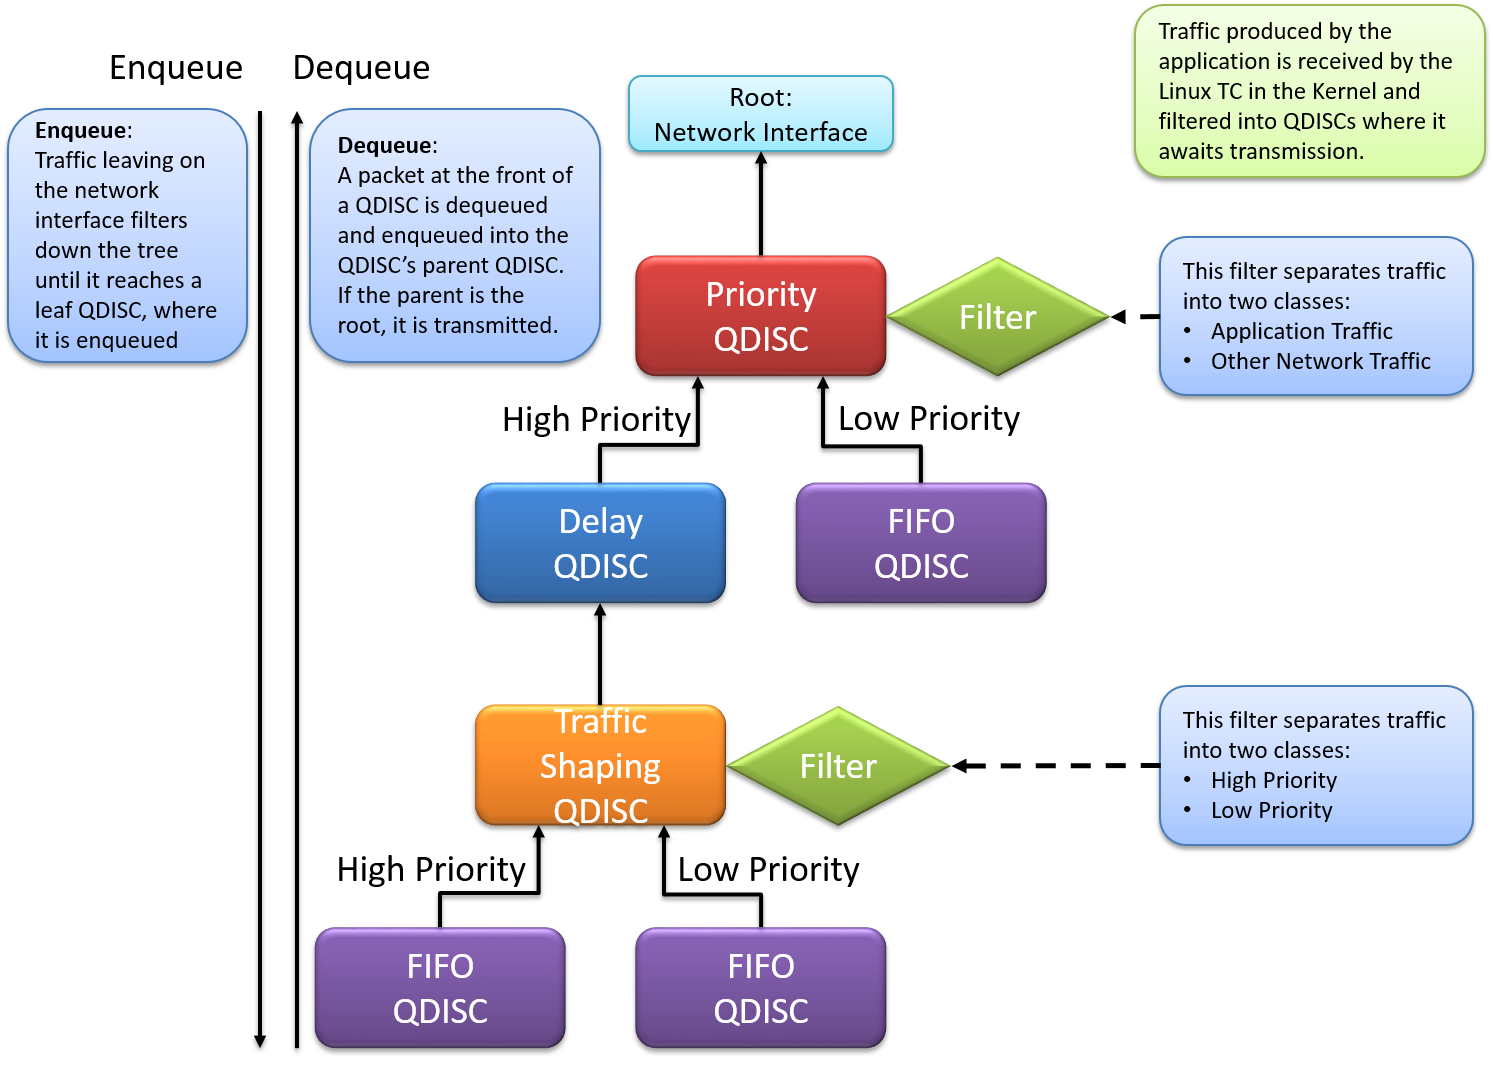
\includegraphics[width=\textwidth]{./figs/tc_diagram.png}
  \caption{Diagram illustrating the TC configuration used to implement
    priority flows, traffic shaping, and delay.}
  \label{fig:tc_diagram}
\end{figure}
